\chapter{Capa de transporte}

\subsubsection{Objetivos}
\begin{itemize}
    \item Comprender las funiconalidades y servicios de la capa de transporte.
        \begin{itemize}
            \item Servicio de multiplexación/demultiplexación.
            \item Servicio orientado a conexión frente a no orientado a conexión.
            \item Cómo conseguir una transferencia de datos fiable.
            \item Cómo proporcionar control de flujo.
            \item Cómo proporcionar control de congestión.
            \item Cómo se han implementado estas funcionalidades en Internet.
        \end{itemize}
\end{itemize}

\section{Introducción}
El nivel de enlace se encarga de ir punto a punto. El nivel de red se encarga de encaminar punto a punto. El nivel de transporte por su parte solo se encarga de la transferencia entre los extremos. Por tanto solo los dispositivos extremos, es decir, normalmente los hosts cuentan con la capacidad de procesamiento a nivel de transporte. \\

Siempre que tengamos el nivel de transporte, tendremos el nivel de aplicación por encima, no tiene utilidad por sí sola la capa de transporte. Por tanto, dentro de un paquete de transporte (datagrama en UDP y segmento en TCP) siempre irá un paquete de aplicación (mensaje).\\

\subsubsection{Funciones y servicios}
\begin{itemize}
    \item Comunicación extremo a extremo.
    \item Multiplexación y demultiplexación de aplicaciones por puertos (cualquier protocolo de transporte debe implementar esta funcionalidad): esto es que en el origen puede entrar en la red información de muchos procesos distintos (multiplexación) y al llegar al destino se distribuye la información entre los procesos necesarios (demultiplexación). Esto se hace a través de puertos. 
\end{itemize}

\begin{definicion}[Puertos]
    Es un número que le dice al SO ``Cuando llegue un paquete por este puerto, está asociado a cierto proceso''. Los puertos que están por debajo de 1024 el SO los ofrece a los usuarios root y los que están por encima están a disposición del desarrollador y no se necesitan permisos de root para utilizarlos. Los puertos de TCP y UDP (que veremos más adelante) son independientes.
\end{definicion}

\begin{description}
    \item [UDP]~\\
        Es un servicio no orientado a conexión, no fiable. Su intención no es ser iable, sino ir rápido.
    \item [TCP]~\\ 
        Es un servicio orientado a conexión, fiable. Hace control de errores, de flujo, de conexión y de congestión. En redes cableadas TCP siempre asume que los errores son por congestión (ya que la tasa de fallo es de 1 entre 1 millón). Sin embargo, en redes inalámbricas sí hay que asumir que puede ser por otras razones (la tasa de fallo es del 10\%).
\end{description}

La velocidad en UDP depende de la aplicación, va sobre una media. En TCP va a la máxima velocidad que puede pero controlando que no haya errores ni pérdidas. 

\section{Protocolo de datagrama de usuario (UDP)}
Es un protocolo ``best effort'' (intenta hacerlo lo mejor posible, pero si hay algún error no intenta solucionarlo). No es orientado a conexión: no hay \textit{hand-shaking}, no hay retardos de establecimiento. Cada paquete es totalmente independiente. Cada \acrlong{TPDU} es independiente. Cada paquete UDP se encapsula en un datagrama IP. \\

Ofrece un servicio no fiable, puede haber pérdidas. Sin embargo esto no significa que no puedan haber aplicaciones fiables sobre UDP, pero quien tiene que encargarse de arreglar los posibles errores es la capa de aplicación.\\

Los datos pueden llegar desordenados (por haber tomado distintos caminos en el encaminamiento, o por distintas prioridades) pero UDP no hace nada para arreglarlo.\\

No hay control de congestión, los datos se \textbf{intentan} entregar lo más rápido posible.\\ 

Lo único que hace UDP (al igual que cualquier protocolo de transporte) es multiplexar y demultiplexar.\\

UDP se usa frecuentemente para aplicaciones multimedia que son tolerantes a fallos y sensibles a retardos. 

\subsection{Cabeceras UDP}
Son 8 Bytes de cabecera. 
\begin{figure}[H]
    \centering
    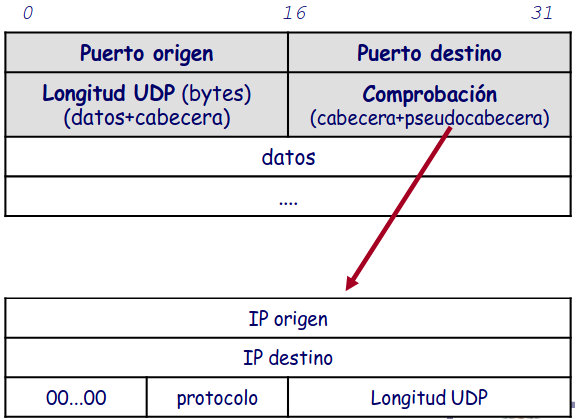
\includegraphics[width=0.6\linewidth]{./images/cabecera-udp.png}
\end{figure}

\begin{itemize}
    \item Puerto origen (16 bits): donde escucha el emisor.
    \item Puerto destino (16 bits): donde escucha el receptor.
    \item Longitud UDP (16 bits): en bytes, datos + cabecera.
    \item Comprobación, checksum (16 bits): no comprueba los datos, sino la cabecera y pseudocabecera, que es una parte de la cabecera IP con datos relevantes para UDP.
        \begin{itemize}
            \item IP origen.
            \item IP destino.
            \item Protocolo.
            \item Longitud UDP.
        \end{itemize}
\end{itemize}

\subsection{Multiplexación/demultiplexación}
Existen puertos preasignados con servicios normalizados:
\begin{figure}[H]
    \centering
    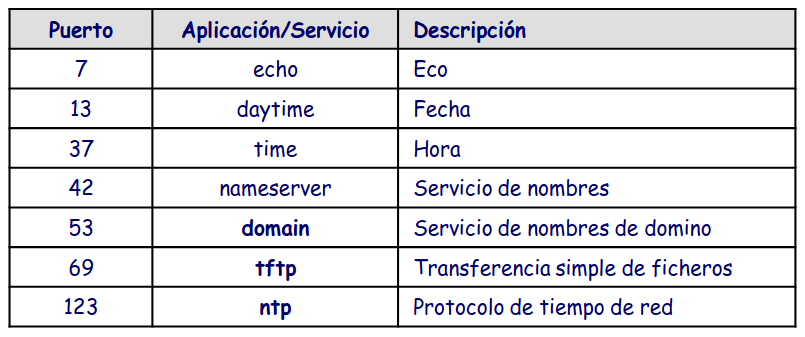
\includegraphics[width=0.6\linewidth]{./images/puertos-udp.png}
\end{figure}


\section{Protocolo de control de transmisión (TCP)}
\begin{itemize}
    \item Es un protocolo punto a punto (UDP no), ya que va desde un origen hasta un destino concreto. Cuando se manda un paquete multicast necesariamente tiene que ser en UDP, puesto que TCP es punto a punto, no puede hablar con muchos. 
    \item Es un servicio orientado a conexión, utiliza un protocolo (hand-shaking, aunque se traduce como protocolo es más bien un intercambio muy específico de mensajes). Exige un estado común entre el emisor y el receptor.
    \item Los datos deben entregarse ordenados (esto no significa que necesariamente lleguen ordenados, pero esto se gestiona de tal forma que parezca que sí para la aplicación que usa los datos).
    \item Es transmisión full-duplex.
    \item Tiene un mecanismo de detección y recuperación de errores, retransmitiendo si es necesario (ARQ). Lo consigue usando confiramaciones, que son positivas (solo confirma lo que ha llegado bien, no se dice nada de lo que ha llegado mal o no ha llegado) y acumulativas (si se ha confirmado hasta cierto byte, entonces todo lo anterior ha llegado bien).
    \item Es un servicio fiable: control de flujo y de congestión.
    \item Usa piggybacking: al mandar una confirmación (ACK) se puede aprovechar y mandar datos a la vez.
\end{itemize}

\subsection{Cabecera TCP}
\begin{itemize}
    \item Puerto origen (16 bits): identifica el puerto del emisor.
    \item Puerto destino (16 bits): identifica el puerto del receptor.
    \item Número de secuencia (32 bits): identifica el byte del flujo de datos enviados por el emisor al receptor que representa el offset del segmento.
    \item Número de acuse de recibo (32 bits): el valor del siguiente número de secuencia que el receptor del segmento espera recibir. De esta forma se confirma todo lo anterior también.
    \item Longitud de cabecera (4 bits): indica el tamaño de la cabecera en palabras de 32 bits. De normal el tamaño es de \textbf{20 bytes}.
    \item Reservado: por si dentro de unos años hacen falta más bits.
    \item Flags:
        \begin{description}
            \item [U:] Urgente. De normal los datos se van introduciendo en el buffer del receptor por la derecha y sacando por la izquierda, buffer circular con ventana deslizante. Pero hay datos urgentes que precisan que este orden no se siga. 
            \item [A:] ACK es una confirmación. Si vale 0 el campo de acuse no es de utilidad.
            \item [P:] Push. En TCP el paquete no se manda a la aplicación hasta que no se llene cierto tamaño. Es más eficiente de esta forma, pero a veces necesitamos que los datos se envíen en un momento preciso y para ello sirve este flag, para decir que se manden los datos.
            \item [R:] Reset. Se resetea la conexión.
            \item [S:] Sincronismo. Esta a 1 en el momento del establecimiento de conexión.
            \item [F:] Fin. Cuando está a 1 es porque quiero terminar la conexión. 
        \end{description}
    \item Ventana ofertada para el control de flujo (16 bits): nos indica cuanto espacio libre le queda al buffer del receptor. 
    \item Comprobación (16 bits): incluye cabecera y datos. 
    \item Puntero de datos urgentes (16 bits): si el flag \textbf{P} está activo, este campo nos indica donde empiezan los datos urgentes, puesto que puede que no todo el segmento sea urgente.
    \item Opciones: son opcionales (por ejemplo las características de las extensiones de TCP).
\end{itemize}

\subsection{Multiplexación/demultiplexación}
Existen puertos preasignados con servicios normalizados:
\begin{figure}[H]
    \centering
    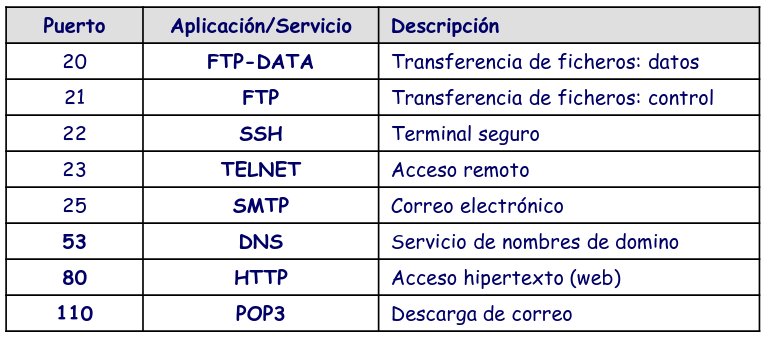
\includegraphics[width=0.6\linewidth]{./images/puertos-tcp.png}
\end{figure}

La conexión TCP se identifica por: puerto e IP origen y puerto e IP destino.
\subsection{Control de conexión}
Como ya hemos comentado, TCP ofrece un servicio orientado a conexión. El intercambio de mensajes tiene tres fases:
\begin{itemize}
    \item Establecimiento de conexión (sincroniza el número de secuencia y se reservan recursos).
    \item Intercambio de datos, full-duplex.
    \item Cierre de conexión, libera recursos.
\end{itemize}

\subsubsection{Establecimiento de conexión}
Se le conoce como ``three-way handshake''. Supongamos que A se quiere comunicar con B. 
\begin{enumerate}
    \item A manda una solicitud a B para activar una conexión, activando para ello el flag de sincronismo y en el campo de secuencia se pone un byte aleatorio X.
    \item Cuando B lo recibe, activa el flag de A (para confirmar el sincronismo) y en el campo de acuse pone X+1 (esto es por convenio). Además, por piggybacking, enviamos el sincronismo en el sentido contrario, activando el bit S y poniendo en el campo de secuencia otro número aleatorio Y.
    \item A recibe esto último y confirma poniendo el flag A a 1 y poniendo en el campo de acuse Y+1. En este mensaje se pueden mandar datos (piggybacking). (Aunque por simplicidad en los ejercicios no lo haremos).
\end{enumerate}
Entonces tenemos que A realiza una \textbf{apertura activa}, siendo el cliente; y B realiza una \textbf{apertura pasiva} siendo el servidor. Los campos que tenemos involucrados son: el bit de sincronismo S, el número de secuencia, el número de acuse, y el bit de ACK A.

La conexión es iniciada siempre por el cliente. Esto se denomina \textbf{apertura activa}. El servidor por su lado siempre está escuchando y cuando le llega una petición hace una \textbf{apertura pasiva}.

\begin{observacion}
    No es posible garantizar un establecimiento de conexión fiable teniendo en cuenta que los mensajes van sobre IP (que no es fiable). Para garantizarlo hay temporizadores y si expiran se reenvían paquetes. 
\end{observacion}

\subsubsection{Número de secuencia}
\begin{itemize}
    \item Es un campo para indicar el orden de los paquetes. Tiene 32 bits. Cuando el número de secuencia llega al máximo ($2^{32}$) se reinicia.
    \item El número de secuencia no empieza normalmente en 0, sino en un valor denominado \acrfull{ISN}, teóricamente aleatorio.
    \item Realmente el ISN es elegido por el SO normalmente. Lo que hace es tener un contador que se va incrementando cada \unit[4]{$\mu s$}. Por lo que tarda en repetirse un ISN casi \unit[5]{horas}.
    \item Este mecanismo de selección de ISN es suficiente para proteger evitar coincidencias, pero no es un mecanismo de protección frente a sabotajes. Es muy fácil averiguar el ISN de una conexión y suplantar a alguno de los participantes.
    \item Se incrementa el número de secuencia de cada segmento según los bytes del segmento anterior. 
    \item Cuando los flags S y F están activados se incrementa en 1 el número de secuencia.
\end{itemize}

Veamos algunos ejemplos de establecimientos de conexión particulares:
\begin{description}
    \item [Establecimiento sin incidencias:]~\\ 
\begin{figure}[H]
    \centering
    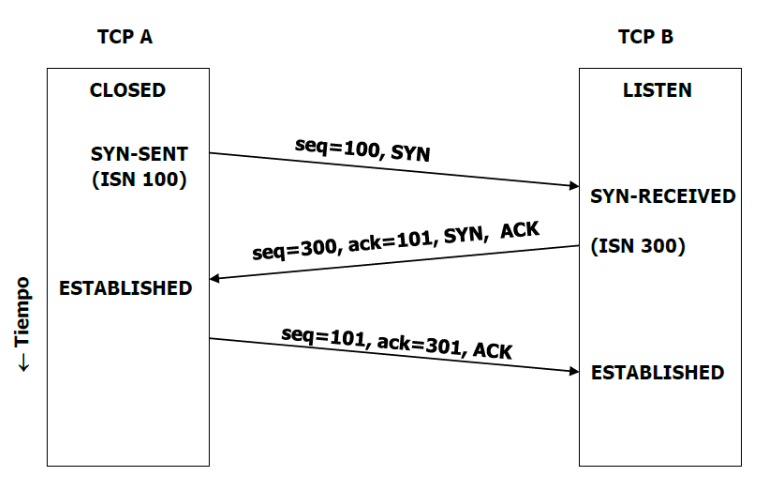
\includegraphics[width=0.6\linewidth]{./images/conexion-normal.png}
\end{figure}
    \item [Caso de conexión simultánea:] En este caso simplemente en el segundo mensaje no es necesario el SYN (pues ya se ha mandado antes).
\begin{figure}[H]
    \centering
    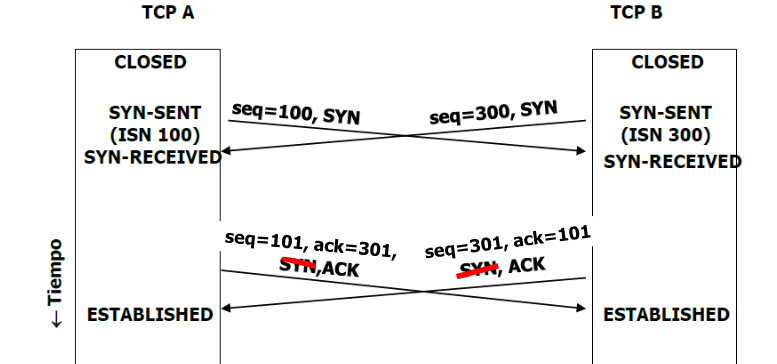
\includegraphics[width=0.6\linewidth]{./images/conexion-simul.png}
\end{figure}
    \item [Caso con SYN retrasados y duplicados:] En este caso cuando el emisor recibe el ACK de la petición que ya ha descartado lo que hace es mandar un mensaje para que el receptor resetee la conexión y ambos estén sincronizados.
\begin{figure}[H]
    \centering
    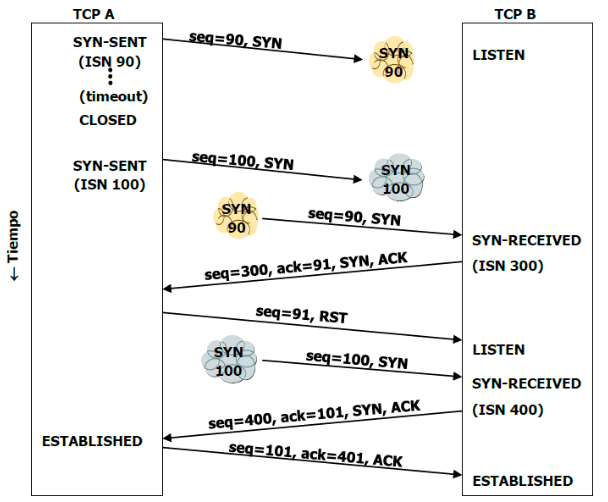
\includegraphics[width=0.6\linewidth]{./images/conexion-retardo.png}
\end{figure}
\end{description}

\subsubsection{Cierre de conexión}
\begin{enumerate}
    \item Se envía un FIN (flag F a 1) y se envía en el número de secuencia el siguiente byte que el otro espera recibir X.
    \item El otro responde con ACK con X+1 y envía un FIN con número de secuencia Y (el siguiente byte que espera recibir el primero).
    \item El primero responde con ACK con Y+1. 
\end{enumerate}

En este caso, al igual que en el establecimiento de conexión, el que inicia el cierre realiza un cierre activo y el otro un cierre pasivo. Dependiendo de la aplicación el cierre activo puede realizarlo tanto el cliente como el servidor.\\

La conexión se cierra, pero para liberar los recursos se deja un tiempo de margen por si tienen que llegar datos aún (suelen ser 2 minutos).

\subsubsection{MSS (Maximum Segment Size)}
El MTU, que es un concepto de capa de enlace (capa 2), especifica la longitud máxima de datos de un paquete de enlace, es decir, cabecera IP + datos IP. \\

MSS es un concepto de la capa de transporte. Indica lo que puede ocupar como máximo los datos de TCP. Por tanto, al MTU le tenemos que quitar lo que ocupa la cabecera IP y la cabecera TCP para calcular el MSS. 

\subsubsection{Diagrama de estados de conexiones TCP}
Un diagrama de estados es un autómata finito de estados TCP desde los cuales puedo hacer una serie de acciones, en las cuales puedo recibir y transmitir datos: a/b equivale a que recibo a y transmito b.

\subsection{Control de errores}
Los campos que tenemos involucrados en el control de errores son:
\begin{itemize}
    \item Número de secuencia.
    \item Campo de acuse.
    \item Bit de ACK.
    \item Campo de checksum (incluye cabecera y datos TCP y pseudocabecera IP). 
\end{itemize}

El sistema que se usa para el control de errores es el de confirmaciones positivas y acumulativas. Si el emisor pierde un ACK tiene que reenviar los datos, independientemente de que se haya perdido el dato o el ACK, tienen el mismo efecto ambos sucesos.\\

Lo que se hace es que el emisor tenga unos timeouts para que si este expira reenviemos el dato si no se ha recibido el ACK. Hay que calcular muy bien los timeouts puesto que si es muy corto se reenviarán datos innecesariamente y si es muy largo tardamos mucho en darnos cuenta del error.\\

Por otra parte tenemos el buffer del receptor. Se va rellenando con los datos que van llegando y se van colocando en orden gracias al número de secuencia, es decir, los datos se introducen por la derecha. Hay que destacar que hay un buffer por cada conexión TCP. Cuando la aplicación pide un dato, el SO saca un paquete de más a la izquierda del buffer. Por esto, decimos que el buffer es una ventana deslilzante, una cola FIFO circular.

\subsubsection{Generación de ACKs}
Vamos a ver situaciones que se dan en el receptor y el comportamiento que sigue a dichas situaciones:   
\begin{enumerate}
    \item Si ocurre una llegada ordenada de segmento, sin discontinuidad, y con todo lo anterior ya confirmado, se retrasa el envío del ACK. Se pone un temporizador a \unit{500}{ms} (este tiempo está estipulado en el correspondiente RFC) y si traspasado ese tiempo no ha llegado otro segmento, en ese momento ya sí se envía el ACK. 
    \item Si tenemos todo en orden, y ocurre una llegada ordenada, sin discontinuidad y hay pendiente un ACK retrasado, se manda inmediatamente el ACK acumulativo. Vemos por tanto que se manda un ACK cada dos segmentos, si va todo bien. 
    \item Supongamos que ahora nos llega un segmento con número de secuencia mayor que el esperado, por lo que tenemos una discontinuidad. En este caso se envía un ACK duplicado, indicando el número de secuencia del siguiente byte esperado.
    \item Supongamos por último que llega un segmento que completa una discontinuidad total (tapa el hueco entero) o parcialmente (tapa parte del hueco). En este caso se manda inmediatamente un ACK con el número de segmento del siguiente byte que se espera.
\end{enumerate}

En el control de flujo veremos alguna situación más que requiere envío de ACKs. 

\subsubsection{Estimación de timeouts}
Dichos timeouts deben adaptarse al \acrlong{RTT}. Este no es un valor fijo pues hay que tener en cuenta el tiempo de transmisión (tiempo que tarda en enviarse un paquete, que depende de la tarjeta), tiempo de propagación (tiempo que tarda desde que se empieza a enviarse el paquete hasta que se empieza a recibir, que depende de la distancia y de la red), tiempo de procesado en un router (depende de la carga de la red). Y todo esto es solo el tiempo de ida, a lo que hay que sumarle el tiempo de vuelta, que es similar. \\

Como enviamos un paquete y recibimos un ACK, podemos medir el \acrshort{RTT}. A esto lo llamamos $RTT_{medido}$. 
\begin{equation*}
    RTT_{nuevo} = \alpha\cdot RTT_{viejo} + (1-\alpha)\cdot RTT_{medido}, \ \alpha \in [0,1]
\end{equation*}
Este es un RTT filtrado, es una media suavizada. 
\begin{equation*}
    Desviacion_{nueva} = (1-x)\cdot Desviacion_{vieja} + x\cdot |RTT_{medido}-RTT_{nuevo}|, \ x \in [0,1]
\end{equation*}
Esta es la desviación instantánea respecto a la media, que se utiliza para procurar cubrir todos los casos. 
\begin{equation*}
    Timeout = RTT_{nuevo} + 4\cdot Desviacion_{nueva}
\end{equation*}

Tenemos un problema con los ACKs repetidos, pero esto se soluciona muy fácilmente (algoritmo de Karn). Se actualiza el RTT solo para los ACKs no ambiguos, pero si hay que retransmitir algún segmento, se duplica el timeout. 

\subsection{Control de flujo}
Es un mecanismo de atrás hacia delante: el receptor le dice al emisor que envíe más o menos datos. Los paquetes que lleguen cuando el buffer está lleno se descartan, lo que supone sobrecargar inútilmente la red. Nuestro objetivo es evitar esto. Es un sistema crediticio, el receptor informa al emisor sobre los bytes autorizados a emitir sin esperar respuesta. \\

Se utiliza el campo de la cabecera ventana, que tiene 16 bits, por lo que esto limita el tamaño de la ventana. 
\begin{equation*}
    ventana \ util \ emisor = ventana \ ofertada \ receptor - bytes \ en \ transito.
\end{equation*}
Es importante que tengamos en cuenta los bytes que ya se han mandado pero de los cuáles no hemos recibido confirmación.\\

Cuando la ventana está llena, el emisor se bloquea hasta recibir un nuevo ACK que confirme que se ha liberado espacio de la ventana. Aquí está la situación que comentábamos antes de la necesidad de envío de ACKs fuera del control de errores.\\

Este ACK es importante, dado que si se pierde el emisor se queda bloqueado. Para evitar esta situación se usa un temporizador de persistencia. Cuando expira dicho temporizador se envía 1 byte para que se fuerce el posible reenvío del ACK. \\

Un problema que puede surgir es el Síndrome de la ventana tonta, que sucede cuando por alguna razón se tiene que mandar un segmento corto, a partir de ahí, lo más probable es que la ventana útil sea similar al tamaño de dicho segmento. Esto hace que se sature la red con muchos segmentos cortos. 

Se puede hacer una posible mejora, usar la ventana optimista, no tomamos la ventana útil ni la ofertada, sino una cosa intermedia. \\ 

Hay dos medios que nos permiten saltarnos el orden:
\begin{itemize}
    \item El bit U (urgente) con el campo puntero.
    \item Solicitar entrega inmediata a la aplicación con el bit P (push).
\end{itemize}

\subsection{Control de congestión}
La velocidad de TCP depende en gran parte de esto. Se manifiesta en pérdidas y/o retrasos de ACKs. Es un problema diferente al control de flujo, involucra la red y los sistemas finales. \\

Tiene una naturaleza adelante-atrás: es el emisor el que decide cuánto se transmite. Por esto, no es necesario ningún campo en la cabecera TCP. 

Lo que se hace es en la fuente limitar de forma adaptable el tráfico generado: reduciendo la velocidad de emisión ante congestiones e incrementándola si todo va bien. \\

Primero vamos a explicar el funcionamiento del control de congestión, y luego pasaremos a juntarlo con el control de flujo, dado que están directamente relacionados.

\begin{description}
    \item [Funcionamiento del control de congestión:]~\\
Hablaremos de varios valores: ventana de congestión, ventana inicial y umbral. Aunque realmente lo que mide es la cantidad de bytes hablaremos de cantidad de segmentos. 

En primer lugar se hace el establecimiento de conexión (siempre en TCP). Ahora bien, tras esto, vamos a tener dos fases:
\begin{description}
    \item [Inicio lento:] Al principio la ventana de congestión está puesta en el valor que estipula la ventana inicial (depende del sistema operativo, suele ser 2 para no tener que esperar los \unit{500}{ms}). Se mandan esa cantidad de paquetes, y se espera los ACKs. \\

        Después de cada ACK recibido se le suma a la ventana de congestión anterior la cantidad de paquetes confirmados en dicho ACK. Es decir, si todo va bien, en cada ACK se aumentará la ventana de congestión en 2. Pero si nos damos cuenta, cada \acrshort{RTT} la ventana duplicará su tamaño. Por tanto, la velocidad aumenta exponencialmente.
        \begin{equation*}
            CW = CW + n^o \ datos \ confirmados
        \end{equation*}
        Siempre debemos tener en cuenta que el número de segmentos que podemos enviar es el que nos permite la ventana de congestión menos los segmentos que hay ya en tránsito (al igual que en el control de flujo). 
        Esto va ocurriendo hasta que llegamos a un umbral, y pasamos a la siguiente fase.
    \item [Prevención de congestión:] En esta fase, después de cada confirmación se aumenta la ventana de la siguiente forma:
        \begin{equation*}
            CW = CW + \frac{1}{CW}
        \end{equation*}
        Entonces, cuando pasa un \acrshort{RTT} aumenta en 1 la ventana de congestión, es decir la velocidad aumenta linealmente. 
    \item [Ocurre un timeout:] esto es por que ha habido algún error, y se asume que es por congestión, por lo que volvemos al valor de la ventana inicial y el umbral se establece en la mitad del valor de la ventana de congestión. 
        \begin{equation*}
            \text{umbral} = \frac{CW}{2}, \qquad CW = CW_{inicial}
        \end{equation*}
        En este caso, la ventana de congestión se va a ir duplicando de nuevo, pero ahora de forma más lenta.
\end{description}

    \item [Funcionamiento del control de flujo y congestión:] habiendo explicado ambos funcionamientos por separado, solo nos queda juntarlo. En realidad no solo vamos a tener una de las dos limitaciones aisladas, sino que las tenemos las dos a la vez, por tanto los bytes permitidos a enviar son el mínimo de las dos ventanas, la de congestión y la del receptor.
        \begin{equation*}
            Ventana \ util = \min\{VentanaCongestion, VentanaReceptor\}
        \end{equation*}
\end{description}

\section{Extensiones TCP}
TCP se define con múltiples ``sabores'' o \textit{flavours} en inglés, que no afectan a la interoperabilidad entre los extremos. 
\begin{itemize}
    \item TCP Tahoe: es el que hemos estudiado.
    \item TCP Reno: es la siguiente versión a TCP Tahoe. Distingue entre los timeout, que opera igual que Tahoe, y ACKs duplicados, que pone a la mitad la ventana de congestión y sigue en prevención de congestión. 
    \item TCP NewReno: la versión anterior tiene un inconveniente. Si se pierden muchos paquetes, en cada uno se reduce la ventana a la mitad, cuando realmente esto no es necesario porque probablemente reduciendo una vez hubiera sido diferente. Esta nueva versión intenta ponerle solución a esto con ACKs parciales. 
    \item TCP Vegas: si el \acrshort{RTT} aumenta se disminuye la ventana, y si el \acrshort{RTT} disminuye se aumenta la ventana de congestión.
    \item TCP Cubic: se usa en cualquier versión de Linux con kernel mayor que la 2.6.19. La ventana de congestión depende de los ACKs y del \acrshort{RTT}. 
    \item TCP Westwood: hay que tener en cuenta que, si bien en redes cableadas suponer que los errores siempre son por congestión es un buen enfoque; en redes inalámbricas no es ni de cerca el mejor, pues el 10\% de los errores son por el medio. Esta versión tiene en cuenta esto, y está pensada para redes inalámbricas.
\end{itemize}

